\chapter{Estrategia general del análisis}
\label{cap:estrategia}

En el \cref{cap:estadistica} se describieron los conceptos básicos de estadística
necesarios para poder realizar un análisis de búsqueda de nueva física. En este
Capítulo, haciendo uso de estos conceptos, se describe la estrategia general
y la construcción del modelo estadístico utilizado en el análisis.

%% Como se ha mencionado en el \cref{cap:susy}, debido al gran número de parámetros
%% libres en los modelos de SUSY, las búsquedas de supersimetría en ATLAS están
%% impulsadas por la fenomenología de los estados finales.

El análisis realizado para esta Tesis consiste en la búsqueda de Supersimetría
en eventos con un fotón aislado muy energético, jets y gran cantidad de energía
faltante. La estrategia general consistió en un experimento de conteo, es decir,
considerando el número de eventos observado en una cierta región del espacio de
observables. Un experimento de conteo puede pensarse en el contexto del
likelihood extendido, \cref{eq:likelihood_ext}, con $f(x) = 1$, el cual se
reduce solo al término de Poisson. En el caso de que el número de eventos
observado sea compatible con el número de eventos esperado debido a procesos del
SM, pueden establecerse límites en la sección eficaz de nueva física. En
particular en esta Tesis, se consideró un modelo de Supersimetría que puede dar
lugar a este tipo de estados finales, y también se darán resultados independientes
de cualquier modelo.

%% Para poder determinar compatibilidad entre los eventos observados con los
%% predichos es necesario
Para poder realizar cualquier descubrimiento de nueva física es fundamental entender
y tener bajo control los fondos del SM.
Existen muchos procesos del SM que pueden dar lugar a una estado final con un fotón,
jets y energía faltante. Estos pueden dividirse en varias categorías. Por un lado, los
procesos que dan lugar a eventos con un fotón y energía faltante real, es decir, los
que llamamos fondos irreducibles son:

\begin{itemize}
\item $Z(\to\nu\nu)+\gamma$
\item $W(\to e\nu)+\gamma$, $W(\to\mu\nu)+\gamma$ y $W(\to \tau\nu)+\gamma$ %(con decaimiento hadronico del $\tau$)
\item $t\bar{t}+\gamma$ %(cuando el $e/\mu$ (si se produce) no es reconstruido)
\end{itemize}
%
También es posible que, aunque el proceso no tenga fotones en el estado final, un
electrón o un jet sean identificados como un fotón, dando lugar a un estado final
idéntico al buscado. En esta categoría están:

\begin{itemize}
\item $W(\to l\nu)$ + jets
\item $Z(\to \nu\nu)$ + jets
\item $t\bar{t}$
\item $WW$, $ZZ$, $WZ$
\end{itemize}

Y por último, también podemos tener procesos que a pesar de no generar energía
faltante real, poseen lo que se denomina energía faltante instrumental,
proveniente generalmente de la incorrecta reconstrucción de la energía de los
jets. De esta manera, pueden dar lugar a eventos con el estado final de interés,
los procesos QCD de $\gamma+$jets y multijet (este último con alguno de los jets
identificado como fotón) y también $Z(\to ll)+$jets, donde un leptón o un jet es
identificado como un fotón.


%% \begin{itemize}
%% \item {\MET} real (EWK)
%%   \begin{itemize}
%%   \item $\gamma$ real
%%     \begin{itemize}
%%     \item $Z(\to\nu\nu)+\gamma$
%%     \item $W(\to\tau\nu)+\gamma$, con decaimiento hadronico del $\tau$
%%     \item $W(\to e\nu)+\gamma$, donde el $e$ no es reconstruido
%%     \item $W(\to\mu\nu)+\gamma$ y $W(\to\tau\nu)+\gamma$, el $\mu/\tau$ no es reconstruido
%%     \item $t\bar{t}+\gamma$, donde el $e/\mu$ (si se produce) no es reconstruido
%%     \end{itemize}

%%   \item Electron/Jet mal identificado como un fotón
%%     \begin{itemize}
%%     \item $W(\to l\nu)$+jets
%%     \item $Z(\to \nu\nu)+$jets
%%     \item $t\bar{t}$
%%     \item dibosons
%%     \end{itemize}
%%   \end{itemize}

%% \item {\MET} instrumental
%%   \begin{itemize}
%%   \item $\gamma$ real
%%     \begin{itemize}
%%     \item  ($\gamma+$jets)
%%     \end{itemize}
%%   \item Electron/jet mal-identificado como $\gamma$
%%     \begin{itemize}\itemsep0.2cm\parskip0.2cm
%%     \item multijet
%%     \item $Z(\to ll)+$jets)
%%     \end{itemize}
%%   \end{itemize}

%% \end{itemize}

%% En el \cref{cap:simulaciones} se describen como estos procesos del SM son
%% simulados utilizando generadores Monte Carlo. Aunque en general, para el LHC,
%% las predicciones de las simulaciones Monte Carlo no son lo suficientemente
%% precisas, ya que nunca fueron testeadas a energías tan altas. Por este motivo
%% resulta necesario desarrollar técnicas de estimación de los fondos utilizando los
%% propios datos observados. Estos métodos se describen en el \cref{cap:fondos}.





%---------------
% Regiones
%---------------
\section{Regiones de Señal, Control y Validación}
\label{sec:regiones}

%---------------
% Signal Region
%---------------
Un análisis en el que se quiera estudiar un determinado fenómeno de nueva física
requiere la definición de una región en el espacio de observables, donde el modelo de señal
predice un exceso significativo de eventos sobre el nivel de fondo predicho en
la misma región. A esta región enriquecida en señal se la llama región de señal
(SR).

%-----------
% Fondos/CR
%-----------
Una de las tareas fundamentales del análisis es entonces, estimar las
contribuciones de los procesos del SM (lo que llamamos fondos) que contaminan la región de
señal.
Para esto existen dos técnicas principales: utilizar directamente simulaciones Monte Carlo,
o utilizar métodos basados en los propios datos observados.

%% La primera de las técnicas consiste en generar una gran cantidad de eventos
%% utilizando técnicas de Monte Carlo del proceso físico considerado. En general
%% este proceso se realiza en varias etapas. Con un generador de eventos se realiza
%% la simulación de la interacción fuerte (por ej. {\madgraph}). Luego con el mismo
%% u otro generador se realiza la lluvia de partones y el proceso de hornecino
%% (por ej. {\pythia}). Y finalmente se simula la interacción de las partículas
%% generadas con el detector ({\geant}). A cada proceso que se simula de esta forma
%% lo llamaremos muestra en referencia a la muestra correspondiente generada con
%% Monte Carlo.

%% Para cada proceso físico tenemos que el numero de eventos esperado por unidad de
%% tiempo (tasa) estará dado por:

%% \begin{equation}
%%   \text{tasa} = (\text{flujo}) \times (\text{sección eficaz}) \times
%%   (\text{eficiencia}) \times (\text{aceptancia})
%% \end{equation}
%% %
%% donde la sección eficaz esta predicha por la teoría, el flujo es controlado por
%% el acelerador, y la eficiencia y la aceptancia son propiedades del detector y
%% los criterios de la selección de eventos. Esta relación no es mas que la
%% refórmalo invariante de la probabilidad de dispersión predicha por primeros
%% principios de la mecánica cuántica $P(i\to f) =
%% |\braket{i}{f}|^2/(\braket{i}{i}\braket{f}{f})$.

%% Si llamamos seccion eficaz efectiva $\sigma_\text{eff}$ al producto de la
%% sección eficaz, la eficiencia y la aceptancia, el numero de eventos esperado
%% para un dado proceso ($\nu$) va a ser el producto de la luminosidad integrada en
%% el tiempo $L$ y la sección eficaz efectiva:

%% \begin{equation}
%%   \nu = L \sigma_\text{eff}
%% \end{equation}

%% Sin tener en cuenta los efectos del detector, la distribución de un observable
%% $x$ sera

%% \begin{equation}
%%  f(x) = \frac{1}{\sigma_\text{eff}} \frac{d\sigma_\text{eff}}{dx}
%% \end{equation}

%% Como ya hemos simulado el pasaje de las partículas por el detector podemos
%% estimar la distribución subyacente $f(x)$ creando un histograma del observable
%% $x$ con la muestra simulada.

La validez de la simulaciones MC está fundamentalmente relacionada a cómo la
teoría subyacente modela las observaciones experimentales. Las debilidades de la
estimación del fondo a partir de las simulaciones derivan de las debilidades de
los modelos teóricos propiamente dichos. En este caso existe una motivación para
utilizar métodos que puedan dar una estimación de los fondos a partir de los
datos experimentales. Existen distintas formas para estimar un fondo a partir de
los datos observados. En el \cref{cap:fondos} se describirán los métodos
específicos utilizados en este análisis.

%% En el caso de que no se puedan estimar utilizando los datos, existe una tercera
%% forma
En algunos casos se utiliza un tercer método para estimar los fondos, que consiste en
utilizar la estimación proveniente de las simulaciones MC, pero corregida
utilizando los datos. Para esto se define una región de control (CR) en
la cual el fondo dominante pueda ser controlado comparándolo con los datos
observados en esa misma región. Las CR son diseñadas especialmente para tener
una alta pureza en uno de los procesos de fondo y deben estar libres de
contaminación de señal.

A través del ajuste a los datos, el número de eventos observado en una CR es
usado para normalizar el número de eventos estimado de fondo en todas las
regiones, especialmente en la SR. Es decir, las predicciones iniciales de las
simulaciones MC son llevadas al nivel observado en la correspondiente CR,
usando un factor de normalización calculado en el ajuste. Este factor es
utilizado entonces en la extrapolación a las demás regiones.

%--------------------
% Validation regions
%--------------------
Otro componente importante del análisis es la validación del método utilizado
para predecir los fondos en las SR. Con este objetivo se definen regiones de
validación (VR) que se encuentren entre las CR y las SR en términos de los
principales observables cinemáticos en los criterios de selección. El diseño de
las VR comprende un compromiso entre minimizar la contaminación de la señal, y a su
vez ser efectivas en la validación de la extrapolación entre CR y SR. En la
\cref{fig:regions_sketch} se puede ver un esquema de las regiones descriptas
anteriormente.

\begin{figure}[!htbp]
  \centering 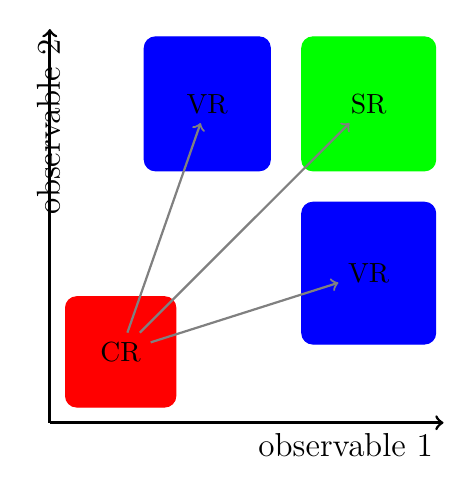
\begin{tikzpicture}

  \tikzstyle{region} = [rounded corners, fill]


  \draw[line width=1, ->] (0,0) -- (5,0) node[below left] {\large observable 1};
  \draw[line width=1, ->] (0,0) -- (0,5) node[left=0.5,rotate=90] {\large observable 2};

  \draw[region, red] (0.2,0.2) rectangle (1.6,1.6) node[midway,black] (CR) {CR};

  \draw[region, green] (3.2,3.2) rectangle (4.9,4.9) node[midway,black] (SR) {SR};

  \draw[region, blue] (3.2,1.0) rectangle (4.9,2.8) node[midway,black] (VR1) {VR};
  \draw[region, blue] (1.2,3.2) rectangle (2.8,4.9) node[midway,black] (VR2) {VR};

  \draw[->,gray, line width=0.8] (CR) -- (SR);
  \draw[->,gray, line width=0.8] (CR) -- (VR1);
  \draw[->,gray, line width=0.8] (CR) -- (VR2);

\end{tikzpicture}

  \caption{Esquema del diseño de las regiones de señal (SR), control (CR) y
    validación (VR) en términos de dos observables arbitrarios.}
  \label{fig:regions_sketch}
\end{figure}

Es importante que las CR, VR y SR sean estadísticamente independientes para
poder combinar la pdf que modela cada región en una pdf conjunta. Esto es
fundamental ya que al ajustar los parámetros de la función likelihood se deberá
hacer un ajuste simultáneo, que es importante para poder compartir los
parámetros de los fondos y las incertezas sistemáticas entre las distintas
regiones de forma consistente.


%------------------------
% Extrapolacion CR -> SR
%------------------------
\section{Extrapolación y factores de transferencia}

Una de las suposiciones realizada en la Sección anterior fue que las variables
cinemáticas que se usan para diferenciar CR y SR están bien modeladas después de
haber ajustado la pdf total a los datos en las CR. Una vez que los procesos de
fondo dominantes son normalizados en las CR, las correspondientes modificaciones
en la pdf pueden ser extrapoladas a las VR, las cuales son utilizadas para
verificar la validez de esta suposición inicial. Una vez que se demuestra el
acuerdo entre las predicciones del fondo normalizadas y los datos observados en
las VR, las predicciones del fondo son extrapoladas a las SR.
Es en este oasi que los datos observados en las SR son considerados por primera
vez para el analisis. Este proceso es llamado \emph{unblinding} y es
utilizado para tener confianza en los métodos usados y
evitar utilizar predicciones prematuras y un posible sesgo en el
resultado final.

En este procedimiento se utilizan de forma implícita los
denominados \emph{factores de transferencia}, como se explica a continuación.
Las predicciones de los fondo normalizadas en el ajuste son:

\begin{align}
  N_p^{\text{est}}(\text{CR}) &= \mu_p \times \text{MC}_p (\text{CR})
  \\ N_p^{\text{est}}(\text{SR}) &= \mu_p \times \text{MC}_p (\text{SR})
\end{align}
%
donde $N_p^{\text{est}}(\text{CR})$ y $N_p^{\text{est}}(\text{SR})$ es el número
de eventos estimado para cada proceso de fondo $p$ y
$\text{MC}_p^{\text{est}}(\text{CR})$ y $\text{MC}_p^{\text{est}}(\text{SR})$ es
el número de eventos obtenido de las simulaciones MC. El factor $\mu_p$ es el
factor de normalización obtenido en el ajuste a datos.

%% En el ajuste, los valores estimados de fondo son tipicamente driven por la estadistica de las
%% CRs.

Definiendo $N_p^\text{fit}(\text{SR})$ como el valor ajustado en la CR, podemos
escribir de forma equivalente:

\begin{align}
  N_p^\text{est}(\text{SR}) &= \mu_p \times \text{MC}_p (\text{SR}) \nonumber \\
  &\equiv N_p^\text{fit}(\text{CR}) \times \left[ \frac{\text{MC}_p(\text{SR})}{\text{MC}_p(\text{CR})} \right]
\end{align}

El cociente que aparece dentro de los corchete es llamado \emph{factor de
  transferencia} (TF). Un aspecto importante de los TF es que que las incertezas
sistemáticas de los valores estimados de fondo pueden ser parcialmente
cancelados en la extrapolación. La incerteza total en el número de eventos de
fondo en la SR es por lo tanto una combinación de las incertezas estadísticas en
las CRs y la incerteza sistemática residual de la extrapolación. Por esta razón
las CR suelen definirse con una selección un poco más relajada, para incrementar
la estadística, sin aumentar significativamente la incerteza en los TF, y así
reducir las incertezas en la SR.


%--------
% Modelo
%--------
\section{Construcción del modelo estadístico}

%% \note{Algo asi?}
%% El modelo, que es simplemente una familia de pdfs despcripta por un numero finioto
%% de parametros, describe la prediccion nominal (junsto con sus variaciones sistematicas
%% asociadas) de las multiples senales y procesos de fondo en las multiples regiones.

%% El modelo estadistico (la pdf)  tiene que contenter el parámetro de interés (la intensidad
%% de la señal $\mu_s$), los factores de normalización para los procesos de fondo, y los
%% llamados parámetros nuisance que modelan el impacto de las incertezas
%% sistemáticas. Cada incerteza sistemática $i$ se describe con un parámetro
%% nuisance $\theta_i$ que interpola entre el valor nominal y las variaciones de
%% las incertezas sistemáticas.

%% Es decir para las variaciones de las incertezas
%% sistemáticas $\pm \sigma$ tenemos $\theta_i = \pm 1$ y $\theta_i = 0$ para el
%% valor nominal.

La función likelihood general para un experimento de conteo como el que se utiliza
en el análisis de esta Tesis es el producto de los términos de Poisson del
número de eventos en la SR y las CR, y una distribución adicional que implementa
las restricciones en las incertezas sistemáticas. Puede escribirse como:

\begin{align}
  L(\mu_s, \bm{\mu}_p, \btheta) &= \mathcal{P}_\text{SR} \, \times \, \mathcal{P}_\text{CR} \, \times \,
  \mathcal{C}_\text{syst} \nonumber \\
  &= \Pois(n|\lambda(\mu_s, \bm{\mu}_p, \btheta)) \, \times \, \prod_{i \in \text{CR}}
  \Pois(n_i|\lambda_i(\mu_s, \bm{\mu}_p, \btheta)) \times C_\text{syst} (\btheta^0, \btheta) \label{eq:model}
\end{align}
%
Los primeros dos factores ($\mathcal{P}_\text{SR}$ y $\mathcal{P}_\text{CR}$)
reflejan las distribuciones de Poisson de $n$, $n_i$, el número de eventos observado
en cada región. Los valores esperados de las distribuciones de Poisson $\lambda_i$ son
funciones que dependen de las predicciones de señal y los distintos fondos $p$,
los parámetros nuisance que parametrizan las incertezas sistemáticas $\btheta$,
los factores de normalización para los procesos de fondo $\bm{\mu}_p$ y también
la intensidad de la señal $\mu_s$. Para $\mu_s = 0$ tenemos la
función likelihood para la hipótesis de solo-fondo y con $\mu_s = 1$ el
valor esperado de señal. %% para el valor nominal de modelo bajo consideración.

Las incertezas sistemáticas son incluidas usando la pdf
$C_\text{syst}(\btheta^0, \btheta)$, donde $\btheta^0$ son los valores centrales
de las medidas auxiliares alrededor de los cuales $\btheta$ puede variarse al
maximizar el likelihood. El impacto de los cambios en los parámetros nuisance,
en los valores esperados están completamente descriptos por las funciones que
predicen la cantidad de señal y fondo, $\lambda_i$. Para parámetros nuisance
independientes $C_\text{syst}$ es simplemente el producto de las pdf
correspondientes a las mediciones auxiliares que describen cada una de las
incertezas sistemáticas, típicamente una distribución gaussiana $G$ con ancho
unidad,

\begin{equation}
  C_\text{syst} (\btheta^0, \btheta) = \prod_{j \in \text{S}} G(\theta_j^0 -
  \theta_j)
\end{equation}
%
donde $S$ es el conjunto completo de las incertezas sistemáticas consideradas. Las
medidas auxiliares $\theta^0_j$ son típicamente fijadas a cero, pero pueden
variar cuando se generan los pseudo-experimentos.


%% \section{Ajustes}

%% \subsection{Ajuste solo-fondo}

%% El proposito es estimar el fondo total en las SR y VR, sin hacer ninguna
%% suposiscion del modelo de senal. Solo se utilizan las muestras de fondo en el
%% modelo. Las CR se suponene  libres de contaminacion de senal y el ajuste
%% solo se realiza en las CR y los procesos de fondo dominantes se normalizan al
%% numero de eventos observados en esas regiones. Se utilizan la ec {\XXX} sin el termino
%% de la SR.

%% Se comparten todos los parametros del ajuste, por lo tanto se usan para predecir
%% el numero de eventos de fondo en SR y VR.

%% Estas predicciones de fondo son independientes del numero de eventos observado
%% en la SR (y VR) ya que solo las CR se usan en el ajuste. Esto permite una
%% comparasion no sesgada entre las predicciones y el numero de evnetos observado
%% en esas regiones.

%% \section{Fit}

%% Analyses generally rely on external predictions for the various background and signal components
%% in the data to aid the interpretation of observations, where the signal component describes the
%% process of interest. In particle physics, simulations of known and hypothesized physics processes
%% are run through a detailed detector simulation, and are subsequently reconstructed with the same
%% algorithms as the data. In addition, background samples can be constructed using data-driven
%% methods. The simulated samples may depend on one or many model parameters, for example the
%% masses of hypothesized new particles such as foreseen by supersymmetry. It may be required, for
%% instance when signals are analyzed over a multi-dimensional space of model parameters, to sample
%% from a “grid” of potential signal scenarios, with each point on that grid corresponding to a unique
%% point in the multi-dimensional parameter space. If no excess is observed in the data, exclusion
%% limits may be set within this grid, excluding a subset of the tested parameter values.
